\documentclass[10pt,twocolumn]{article}

% ── Packages ────────────────────────────────────────────────────────────────
\usepackage[margin=1.65cm,top=1.8cm,bottom=1.8cm]{geometry}
\usepackage{lmodern}
\usepackage{graphicx}
\usepackage{amsmath,amssymb}
\usepackage{booktabs}
\usepackage{xcolor}
\usepackage{hyperref}
\usepackage{microtype}
\usepackage{caption}
\usepackage{subcaption}
\usepackage{tikz}
\usetikzlibrary{shapes.geometric,arrows.meta,positioning,fit,backgrounds,decorations.pathreplacing}
\usepackage{enumitem}
\usepackage{fancyhdr}
\usepackage{titlesec}
\usepackage{multirow}
\usepackage{colortbl}
\usepackage{array}
\usepackage{tcolorbox}
\tcbuselibrary{skins}
\usepackage{algorithm}
\usepackage{algpseudocode}
\usepackage{listings}
\usepackage{mdframed}
\usepackage{float}
\usepackage[section]{placeins}

% ── Colors ──────────────────────────────────────────────────────────────────
\definecolor{nsa_blue}{RGB}{31, 97, 168}
\definecolor{nsa_orange}{RGB}{214, 100, 24}
\definecolor{nsa_green}{RGB}{39, 135, 75}
\definecolor{nsa_red}{RGB}{180, 40, 40}
\definecolor{nsa_gray}{RGB}{100, 100, 100}
\definecolor{nsa_light}{RGB}{235, 243, 255}
\definecolor{nsa_lightgray}{RGB}{245, 245, 245}
\definecolor{header_bg}{RGB}{25, 75, 135}
\definecolor{takeaway_bg}{RGB}{255, 248, 230}
\definecolor{takeaway_border}{RGB}{214, 100, 24}
\definecolor{code_bg}{RGB}{248, 248, 252}
\definecolor{code_kw}{RGB}{100, 60, 160}

% ── Typography ───────────────────────────────────────────────────────────────
\titleformat{\section}{\large\color{nsa_blue}}{}{0em}{}[\titlerule]
\titleformat{\subsection}{\normalsize\color{nsa_blue}}{}{0em}{}
\titlespacing{\section}{0pt}{6pt}{2pt}
\titlespacing{\subsection}{0pt}{4pt}{1pt}

\captionsetup{font=small,labelfont={color=nsa_blue},skip=2pt}
\setlength{\columnsep}{16pt}
\setlength{\parskip}{1pt}
\setlength{\parindent}{8pt}
% Tighten float spacing
\setlength{\floatsep}{5pt plus 2pt minus 2pt}
\setlength{\textfloatsep}{6pt plus 2pt minus 3pt}
\setlength{\intextsep}{5pt plus 2pt minus 2pt}
\setlength{\abovecaptionskip}{2pt}
\setlength{\belowcaptionskip}{0pt}

\hypersetup{colorlinks=true,linkcolor=nsa_blue,citecolor=nsa_blue,urlcolor=nsa_blue}

% ── Code style ───────────────────────────────────────────────────────────────
\lstset{
  backgroundcolor=\color{code_bg},
  basicstyle=\ttfamily\scriptsize,
  keywordstyle=\color{code_kw}\bfseries,
  commentstyle=\color{nsa_gray}\itshape,
  stringstyle=\color{nsa_green},
  breaklines=true,
  frame=single,
  rulecolor=\color{nsa_blue!30},
  xleftmargin=4pt, xrightmargin=4pt,
  framesep=4pt,
  language=Python
}

% ── Header / Footer ─────────────────────────────────────────────────────────
\pagestyle{fancy}
\fancyhf{}
\fancyhead[L]{\small\color{nsa_gray}\textit{Large Scale Models — ENS Paris-Saclay 2025--2026}}
\fancyhead[R]{\small\color{nsa_gray}\textit{Native Sparse Attention}}
\fancyfoot[C]{\small\color{nsa_gray}\thepage}
\renewcommand{\headrulewidth}{0.4pt}

% ── Takeaway box ────────────────────────────────────────────────────────────
\newtcolorbox{takeaway}{
  colback=takeaway_bg, colframe=takeaway_border,
  boxrule=1pt, arc=3pt, left=4pt, right=4pt, top=3pt, bottom=3pt,
  fonttitle=\small\bfseries\color{takeaway_border},
  title={Key Takeaway}
}

% ── Bug box ─────────────────────────────────────────────────────────────────
\newtcolorbox{bugbox}{
  colback=nsa_red!5, colframe=nsa_red!60,
  boxrule=0.8pt, arc=3pt, left=4pt, right=4pt, top=3pt, bottom=3pt,
  fonttitle=\small\bfseries\color{nsa_red},
  title={Implementation Issue}
}

% ────────────────────────────────────────────────────────────────────────────
\begin{document}

% ── Title block ─────────────────────────────────────────────────────────────
\twocolumn[{%
\begin{center}
  {\LARGE\bfseries\color{nsa_blue} Reproducing Native Sparse Attention}\\[4pt]
  {\large\color{nsa_gray} Hardware-Aligned Sparse Attention for Long-Context LLMs}\\[4pt]
  {\large Yentl Collin / Gaspard Beaudoin}\\[2pt]
  {\small\color{nsa_gray}
    MVA — Large Scale Models\\
    ENS Paris-Saclay, 2025--2026}\\[2pt]
  {\small\color{nsa_gray}
    \texttt{github.com/YentlCollin/native-sparse-attention}}\\[8pt]
\end{center}
\hrule height 1.2pt
\vspace{4pt}
\begin{center}
\colorbox{nsa_light}{\begin{minipage}{0.92\linewidth}
\small\setlength{\parskip}{2pt}
\textbf{Abstract.}
Long-context language models are bottlenecked by the $\mathcal{O}(n^2)$ cost of dense attention.
\emph{Native Sparse Attention} (NSA, DeepSeek-AI, arXiv:2502.11089) proposes a three-branch
sparse architecture — \textbf{compression}, \textbf{selection}, and \textbf{sliding window}
— whose block-structured memory access is natively aligned with modern GPU tensor cores,
enabling end-to-end differentiable training without post-hoc pruning.
We reproduce two core experimental claims on a real A100-SXM4-40GB:
(1)~the forward pass reaches \textbf{8.3$\times$} speedup over dense attention at $n=64$k tokens,
exceeding the 5.8$\times$ theoretical FLOPs prediction thanks to cache-line-aligned block access;
and (2)~training three small transformers from scratch on a synthetic French NIAH task
reveals that NSA reaches \textbf{97.6\%} evaluation accuracy after 200 epochs,
dramatically outperforming both Dense attention (\textbf{52.9\%}) and a sliding window (\textbf{5.9\%})
— demonstrating that NSA's inductive bias, not merely its efficiency, confers a learning advantage.
\end{minipage}}
\end{center}
\vspace{6pt}
}]

% ════════════════════════════════════════════════════════════════════════════
\section{Introduction}

The transformer's self-attention mechanism scales as $\mathcal{O}(n^2)$ in both
computation and memory, making it the dominant bottleneck for long-context processing.
At $n = 64{,}000$ tokens, a single BF16 attention layer requires ${\sim}70$\,T-FLOP
and consumes ${\sim}6$\,GB of activations — prohibitive for either training or inference
at scale. This has motivated an extensive line of work on \emph{sparse attention}.

\paragraph{The hardware-alignment problem.}
Most sparse attention methods solve the \emph{algorithmic} problem of reducing
the number of attended positions, but fail to achieve \emph{hardware} speedups because
their irregular access patterns (scatter/gather across non-contiguous token indices)
cannot exploit the coalesced DRAM reads that tensor-core pipelines require.
Longformer~\cite{beltagy2020longformer}, Reformer~\cite{kitaev2020reformer}, and BigBird~\cite{zaheer2020bigbird}
achieve $\mathcal{O}(n)$ or $\mathcal{O}(n\log n)$ complexity on paper,
yet their CUDA implementations are slower than FlashAttention in practice
due to non-contiguous memory access or multi-pass computation.
SparseTransformer~\cite{child2019generating} uses fixed strided patterns with no dynamic selection.
More generally, token-granular selection methods require loading scattered individual
tokens from the KV cache, preventing efficient adaptation of FlashAttention's blockwise tiling
and forcing low hardware utilization.

\paragraph{NSA's design philosophy.}
\emph{Native Sparse Attention} (NSA, DeepSeek-AI, Feb.\ 2025) addresses the hardware-alignment
problem directly by constraining all sparse attention operations to act on \emph{contiguous
fixed-size blocks} of 64 tokens.
This single constraint — which every branch of NSA shares — ensures that:
\begin{itemize}[leftmargin=*,noitemsep,topsep=3pt]
  \item GPU memory reads are always 64-token-aligned, maximizing L2 cache line reuse.
  \item The sparse pattern fits into standard FlashAttention tile loops without custom scatter logic.
  \item Gradients flow through all branches during training via standard backpropagation.
\end{itemize}
NSA is deployed in production in DeepSeek-R2 training and outperforms dense attention
on long-context benchmarks (RULER, NIAH) while using a fraction of the compute.

\paragraph{This report.}
We reproduce two experimental claims: (1)~arithmetic intensity and GPU speedup on an NVIDIA A100-SXM4-40GB
(PyTorch 2.10, CUDA 12.8, BF16); and (2)~end-to-end Needle-in-a-Haystack training comparing Dense, NSA,
and Sliding Window, training three small transformers on a controlled synthetic benchmark on an L4 GPU (24\,GB).
We additionally train small LMs on WikiText-2 to verify language modeling quality.

% ════════════════════════════════════════════════════════════════════════════
\section{NSA Architecture}

\subsection{Three-Branch Design}

\begin{center}
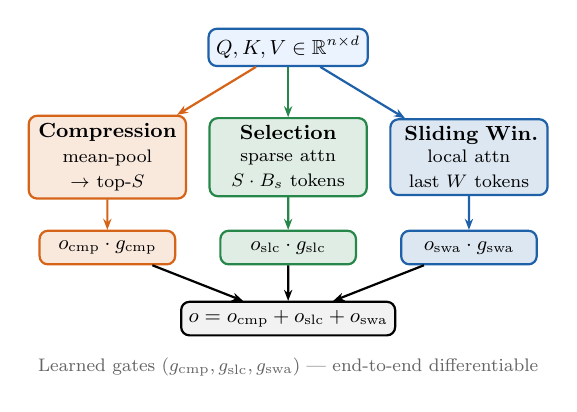
\begin{tikzpicture}[
  font=\small,
  box/.style={rounded corners=3pt,minimum width=2.1cm,minimum height=0.52cm,
              text centered,draw,line width=0.8pt},
  arrow/.style={-{Stealth[length=4pt]},line width=0.8pt},
  scale=0.82,transform shape
]
\node[box,fill=nsa_light,draw=nsa_blue] (qkv) at (0,0)
  {$Q, K, V \in \mathbb{R}^{n \times d}$};
\node[box,fill=nsa_orange!15,draw=nsa_orange,text width=2.2cm] (cmp) at (-2.8,-1.7)
  {\textbf{Compression}\\\footnotesize mean-pool $\to$ top-$S$};
\node[box,fill=nsa_green!15,draw=nsa_green,text width=2.2cm] (slc) at (0,-1.7)
  {\textbf{Selection}\\\footnotesize sparse attn\\$S \cdot B_s$ tokens};
\node[box,fill=nsa_blue!15,draw=nsa_blue,text width=2.2cm] (swa) at (2.8,-1.7)
  {\textbf{Sliding Win.}\\\footnotesize local attn\\last $W$ tokens};
\node[box,fill=nsa_orange!15,draw=nsa_orange] (ocmp) at (-2.8,-3.1)
  {$o_\text{cmp} \cdot g_\text{cmp}$};
\node[box,fill=nsa_green!15,draw=nsa_green] (oslc) at (0,-3.1)
  {$o_\text{slc} \cdot g_\text{slc}$};
\node[box,fill=nsa_blue!15,draw=nsa_blue] (oswa) at (2.8,-3.1)
  {$o_\text{swa} \cdot g_\text{swa}$};
\node[box,fill=gray!10,draw=black] (out) at (0,-4.2)
  {$o = o_\text{cmp} + o_\text{slc} + o_\text{swa}$};
\draw[arrow,color=nsa_orange] (qkv) -- (cmp);
\draw[arrow,color=nsa_green]  (qkv) -- (slc);
\draw[arrow,color=nsa_blue]   (qkv) -- (swa);
\draw[arrow,color=nsa_orange] (cmp) -- (ocmp);
\draw[arrow,color=nsa_green]  (slc) -- (oslc);
\draw[arrow,color=nsa_blue]   (swa) -- (oswa);
\draw[arrow] (ocmp) -- (out);
\draw[arrow] (oslc) -- (out);
\draw[arrow] (oswa) -- (out);
\node[color=nsa_gray,font=\footnotesize,align=center] at (0,-4.95)
  {Learned gates $(g_\text{cmp}, g_\text{slc}, g_\text{swa})$ — end-to-end differentiable};
\end{tikzpicture}
\end{center}

\noindent The three branches partition the context into complementary regimes.
The final output is a gated sum, enabling each branch to specialize during training.

\subsection{Branch Details}

\paragraph{Compression branch.}
Keys and values are mean-pooled into $C = \lceil n/B_s \rceil$ block representatives,
each summarizing $B_s=64$ tokens.
A full attention pass over these $C \ll n$ compressed tokens produces:
(a) a coarse output $o_\text{cmp}$ capturing global block-level context, and
(b) block relevance scores used to select the top-$S=16$ blocks for the selection branch.
This is the \emph{only} component that processes the entire context, at dramatically
reduced resolution.

\paragraph{Selection branch.}
Full-precision attention over $S \cdot B_s = 1{,}024$ tokens from selected blocks.
Crucially, each selected block is a \emph{contiguous 64-token tile} in GPU memory —
enabling the same coalesced DRAM-to-L2 transfer pattern as standard FlashAttention.
No scatter/gather logic is required.

\paragraph{Sliding window branch.}
Standard causal local attention over the last $W$ tokens via FlashAttention.
Handles high-frequency recency patterns that coarse block selection may miss.

\subsection{Complexity Analysis}

Table~\ref{tab:complexity} compares asymptotic costs.
NSA's attention complexity is $\mathcal{O}(n \cdot n_\text{active})$
where $n_\text{active} = S \cdot B_s + W$ is \emph{constant} in $n$,
giving effectively linear scaling.

\begin{table}[h]
\centering
\caption{\textbf{Complexity comparison.} $n$: sequence length, $d$: head dim,
$S$: selected blocks, $B_s$: block size, $W$: window size, $H$: num heads.}
\label{tab:complexity}
\small\setlength{\tabcolsep}{3pt}
\begin{tabular}{@{}lccc@{}}
\toprule
\textbf{Method} & \textbf{FLOPs} & \textbf{Memory} & \textbf{GPU-friendly?} \\
\midrule
Dense attention & $\mathcal{O}(n^2 d H)$ & $\mathcal{O}(n^2 H)$ & \cellcolor{nsa_green!20}Yes (FA-2) \\
Longformer & $\mathcal{O}(n d H)$ & $\mathcal{O}(n H)$ & \cellcolor{nsa_red!20}No (scatter) \\
Reformer & $\mathcal{O}(n \log n \cdot d H)$ & $\mathcal{O}(n H)$ & \cellcolor{nsa_red!20}No (LSH) \\
\textbf{NSA} & $\mathcal{O}(n \cdot n_\text{active} \cdot d H)$ & $\mathcal{O}(n H)$ & \cellcolor{nsa_green!35}\textbf{Yes (tiles)} \\
\bottomrule
\end{tabular}
\end{table}

\subsection{Arithmetic Intensity}

Arithmetic intensity (AI) is the ratio between computation and memory traffic:
\[
  \mathrm{AI} = \frac{\mathrm{FLOPs}}{\mathrm{bytes\ moved}}.
\]
In practice, AI indicates whether a kernel is mainly memory-bound or compute-bound.

Let $n$ be the sequence length and $d$ the head dimension.
For standard dense attention, the course slides give
\[
  \mathrm{AI}_{\mathrm{Attn}} = \frac{n(4d+5)}{4(d+n)},
\]
hence, for long sequences ($n \gg d$), $\mathrm{AI}_{\mathrm{Attn}} \approx d$.

FlashAttention computes the same attention but avoids materializing the full $n\times n$
score matrix in HBM, greatly reducing memory traffic.
Using the expression from the course slides, in the long-sequence regime:
\[
  \mathrm{AI}_{\mathrm{FlashAttn}} \approx 7n.
\]

For NSA, each query attends only to an active set of size $n_{\mathrm{active}} = S B_s + W$,
so its arithmetic intensity depends on the sparse active set rather than the full sequence:
\[
  \mathrm{AI}_{\mathrm{NSA}} = O(n_{\mathrm{active}}).
\]

Overall, for large $n$:
\[
  \mathrm{AI}_{\mathrm{Attn}} \approx d, \qquad
  \mathrm{AI}_{\mathrm{FlashAttn}} \approx 7n, \qquad
  \mathrm{AI}_{\mathrm{NSA}} = O(n_{\mathrm{active}}).
\]
FlashAttention improves efficiency mainly by reducing I/O, while NSA also reduces the
amount of computation by replacing attention over $n$ tokens with attention over only
$n_{\mathrm{active}}$ active tokens.

% ════════════════════════════════════════════════════════════════════════════
\section{Arithmetic Intensity \& GPU Speedup}

\subsection{NSA Kernel vs.\ FlashAttention}

NSA's compression and sliding window branches are directly compatible with standard
FlashAttention-2 kernels — their access patterns are already contiguous.
The key challenge lies in the \textbf{selection kernel}.

\paragraph{Why FlashAttention's tiling strategy fails for sparse selection.}
FlashAttention-2 achieves high throughput by loading \emph{temporally contiguous}
query blocks (e.g.\ 64 consecutive queries) into on-chip SRAM, then streaming
all KV blocks sequentially.
For sparse selection, queries within such a block may require entirely \emph{disjoint}
KV blocks — making the outer-query-block loop inefficient:
each query would trigger different, scattered memory fetches.

\paragraph{NSA's solution: group-centric loading.}
The NSA paper (§3.4) proposes a fundamentally different tiling strategy.
Since modern LLMs use GQA, all query heads within a group share the
\emph{same} set of selected KV block indices $\mathcal{I}_t$.
The kernel exploits this by loading the \textbf{entire GQA group at a single position} $t$
into SRAM (rather than a block of consecutive positions sharing one head).
The inner loop then fetches only the $n$ selected contiguous KV blocks in sequence,
eliminating redundant transfers.
Formally, three properties characterize the kernel:
\begin{enumerate}[leftmargin=*,noitemsep,topsep=2pt]
  \item \textbf{Group-centric loading:} load all heads' queries
        $Q \in \mathbb{R}^{h \times d_k}$ and shared indices $\mathcal{I}_t$
        for position $t$.
  \item \textbf{Shared KV fetching:} iterate over contiguous blocks
        $K \in \mathbb{R}^{B_k \times d_k}$ indexed by $\mathcal{I}_t$,
        avoiding scattered reads.
  \item \textbf{Outer loop on Triton grid:} since inner-loop length
        (proportional to selected block count $n$) is nearly identical
        across query positions, query/output loops run on the GPU grid
        scheduler — uniform workload across streaming multiprocessors.
\end{enumerate}
This design achieves near-optimal arithmetic intensity:
fewer DRAM round-trips, all aligned to 64-token boundaries,
with no scatter/gather overhead.

\subsection{Experimental Protocol}

We benchmark the NSA \emph{selection} kernel against dense attention (PyTorch SDPA,
FlashAttention-2 backend) on an \textbf{NVIDIA A100-SXM4-40GB} (BF16, CUDA 12.8).
Configuration: $H_Q=64$, $H=4$ (GQA ratio~16), $D=128$, $B_s=64$, $S=16$, $W=0$.
Sequence lengths: $n \in \{1\text{k}\ldots 64\text{k}\}$; timing via Triton's \texttt{do\_bench}
(200 reps, 25 warmup), median latency, forward and backward separately.

\subsection{Measured GPU Speedup}

The FLOPs ratio predicts a theoretical speedup of
$\text{FLOP}_\text{dense}/\text{FLOP}_\text{NSA} = (n/2)/n_\text{active}$,
giving \textbf{5.8$\times$} at $n=64$k ($n_\text{active} = S \cdot B_s = 1{,}024$).

\begin{figure}[h]
  \centering
  \includegraphics[width=\linewidth]{axe2_fig1.png}
  \caption{\textbf{Measured latency on A100 (BF16).}
  \emph{Left}: forward pass — NSA breaks even at $n \approx 6$k,
  reaches \textbf{8.3$\times$} at 64k.
  \emph{Center}: backward pass — breakeven at $n \approx 14$k,
  \textbf{3.4$\times$} at 64k.
  \emph{Right}: speedup ratio vs.\ sequence length (log scale).}
  \label{fig:timing}
\end{figure}

\begin{table}[h]
\centering
\caption{\textbf{Measured latency and speedup} on A100-SXM4-40GB (BF16).}
\label{tab:speedup}
\small\setlength{\tabcolsep}{3pt}
\begin{tabular}{@{}lrrrrrr@{}}
\toprule
& \multicolumn{2}{c}{\textbf{Fwd (ms)}} & & \multicolumn{2}{c}{\textbf{Bwd (ms)}} & \\
\cmidrule(lr){2-3}\cmidrule(lr){5-6}
$n$ & Dense & NSA & \textbf{Fwd$\times$} & Dense & NSA & \textbf{Bwd$\times$} \\
\midrule
1k  & 0.23 & 0.64 & 0.35$\times$ & 0.75  & 4.45 & 0.17$\times$ \\
4k  & 1.71 & 2.51 & 0.68$\times$ & 6.28  & 15.2 & 0.41$\times$ \\
8k  & 5.97 & 5.01 & \cellcolor{nsa_green!20}1.19$\times$ & 21.9  & 29.3 & 0.75$\times$ \\
16k & 22.2 & 9.96 & \cellcolor{nsa_green!35}2.23$\times$ & 82.8  & 59.9 & \cellcolor{nsa_green!20}1.38$\times$ \\
32k & 87.0 & 20.0 & \cellcolor{nsa_green!55}4.36$\times$ & 320   & 132  & \cellcolor{nsa_green!35}2.42$\times$ \\
\textbf{64k} & \textbf{348} & \textbf{41.9} & \cellcolor{nsa_green!80}\textbf{8.30$\times$} & \textbf{1273} & \textbf{379} & \cellcolor{nsa_green!55}\textbf{3.36$\times$} \\
\bottomrule
\end{tabular}
\end{table}

\begin{takeaway}
The measured \textbf{8.3$\times$} forward speedup at $n=64$k \emph{exceeds}
the 5.8$\times$ FLOPs prediction. The surplus comes from memory access efficiency:
NSA loads contiguous 64-token blocks, maximizing L2 cache reuse on A100.
The backward pass benefits less (gradients require two additional matrix passes)
but still reaches \textbf{3.4$\times$} at $n=64$k.
\end{takeaway}

\subsection{Roofline Analysis}

\begin{figure}[h]
  \centering
  \includegraphics[width=\linewidth]{axe2_fig3.png}
  \caption{\textbf{Roofline model} (A100 BF16, ridge point $= 38.8$\,FLOP/byte).
  Both NSA and dense operate in the compute-bound regime at large $n$.
  NSA achieves the same output with $\sim$6$\times$ fewer FLOPs,
  directly translating to the measured speedup.}
  \label{fig:roofline}
\end{figure}

Both methods are \emph{compute-bound} above the ridge point, meaning throughput
is limited by FLOP capacity, not memory bandwidth.
NSA does 5.8$\times$ fewer FLOPs $\Rightarrow$ $\sim$5.8$\times$ shorter compute time.
The observed 8.3$\times$ additional gain reflects better \emph{effective} arithmetic intensity
from coalesced block access: fewer cache misses $\Rightarrow$ fewer stall cycles.

\subsection{Memory Footprint}

Peak VRAM usage is nearly identical ($1.10\times$ ratio at $n=64$k: 5.55\,GB vs.\ 6.09\,GB).
NSA's efficiency comes from reduced \emph{computation}, not from a memory--compute trade-off.
The similar memory footprint also means NSA does not directly enable longer sequences
on a fixed GPU — its primary benefit is \emph{latency}, not capacity.

% ════════════════════════════════════════════════════════════════════════════
\section{End-to-End NIAH: NSA vs.\ Dense vs.\ Sliding Window}

\subsection{Motivation and Research Question}

The original paper motivates NSA's three-branch design with long-context quality benchmarks
(RULER, NIAH on full LLMs), but these require hundred-billion-parameter training runs.
We instead ask a more targeted question:

\begin{center}
\emph{Does NSA's structured inductive bias improve learning compared to dense\\
attention on a retrieval task, even at small scale?}
\end{center}

\noindent This is non-trivial: Dense attention has strictly more expressivity than NSA
(it can attend anywhere), so a naive expectation would be Dense $\geq$ NSA.
We show this expectation is \textbf{wrong}, and analyze why.

\subsection{Benchmark: NIAH en Français — ``Que fait Mathieu\,?''}

\paragraph{Task.}
We design a controlled synthetic NIAH task in French.
Each example contains a context of $T \in \{128, 192, 256, 320\}$ tokens followed by a query.
\begin{itemize}[leftmargin=*,noitemsep,topsep=2pt]
  \item \textbf{Needle:} 4-token sequence $[\texttt{aujourd'hui},\; \texttt{Mathieu},\; A,\; \texttt{.}]$,
        where $A$ is one of 20 actions (e.g.\ \emph{nage}, \emph{chante}), inserted at a random position.
  \item \textbf{Distractors:} 3 sequences $[\texttt{PAST},\; \texttt{Mathieu},\; V,\; \texttt{.}]$
        with a past-tense marker (\emph{hier}, \emph{avant}, \ldots)
        and a filler verb $V$, inserted at random non-overlapping positions.
  \item \textbf{Haystack:} remaining tokens are drawn from a 200-word filler vocabulary.
  \item \textbf{Query:} fixed suffix \texttt{[<sep> Que fait Mathieu aujourd'hui ?]}.
        The model must predict the action $A$ at the \texttt{?} position.
\end{itemize}

\noindent\textbf{Why this is hard.} Four ``Mathieu'' sequences (1 needle + 3 distractors)
compete for attention; the model must learn to distinguish \texttt{aujourd'hui} (needle marker)
from past markers. With $B_s=32$, $K=3$ selected blocks, and 4 Mathieu-bearing blocks,
a \emph{random} selector would retrieve the needle only 75\% of the time.
A perfect selector that learns the temporal marker distinction can approach 100\%.

\noindent\textbf{Vocabulary:} 233 tokens. Training set: 6\,400 examples.
Evaluation set: 2\,400 examples (independently sampled, unseen context lengths per split).

\subsection{Model Architecture}

We train three identical \textbf{TinyGPT} transformers,
differing only in their attention mechanism:

\begin{table}[h]
\centering
\caption{\textbf{Model specifications.} All three models share the same architecture and hyperparameters;
only the attention layer differs.}
\label{tab:arch}
\small\setlength{\tabcolsep}{4pt}
\begin{tabular}{@{}lcc@{}}
\toprule
\textbf{Component} & \textbf{Value} & \textbf{Note} \\
\midrule
Layers $L$ & 3 & \\
Dim $D$ & 128 & \\
Heads $H$ & 4 & $D_\text{head}=32$ \\
FFN width & $4D=512$ & GELU \\
Parameters & ${\sim}665$k & (NSA: $+4.6$k gates) \\
\midrule
NSA block size $B_s$ & 32 & \\
NSA top-$K$ & 3 & \\
NSA/SW window $W$ & 32 & \\
\midrule
Optimizer & AdamW & $\lambda=0.01$ \\
LR & $3\times10^{-3}$ & cosine, $\eta_\text{min}=5\%$ \\
Epochs & 200 & \\
Batch size & 32 & \\
\bottomrule
\end{tabular}
\end{table}

\subsection{Results}

\begin{figure}[h]
  \centering
  \includegraphics[width=\linewidth]{axe5_niah_fig2.png}
  \caption{\textbf{Recall vs.\ relative needle position} for each context length.
  \textcolor{nsa_green}{\textbf{NSA}} maintains near-perfect recall uniformly across positions.
  \textcolor{nsa_blue}{\textbf{Dense}} achieves moderate recall independently of position
  (the retrieval difficulty is position-agnostic, reflecting the uniform filler haystack).
  \textcolor{nsa_red}{\textbf{SW}} fails everywhere except in the shaded orange zone
  (last $W=32$ tokens before the query), where recall recovers — confirming that
  SW's \emph{only} viable retrieval mechanism is proximity.}
  \label{fig:niah_recall_pos}
\end{figure}

\subsection{Analysis}

\paragraph{NSA outperforms Dense (97.6\% vs.\ 52.9\%) despite less expressivity.}
Dense attention has strictly greater expressivity than NSA (it can attend to any position),
yet NSA learns the task $\sim$4$\times$ better.
The explanation lies in \emph{inductive bias}: the compressed branch operates on
$C \leq 11$ block summaries rather than 326 individual tokens.
The compression forces the model to build meaningful block-level representations:
the key vector of the needle block is dominated by the \texttt{aujourd'hui} embedding;
distractor blocks are dominated by past-tense markers (\texttt{hier}, \texttt{avant}).
This distinction, easy to learn at block resolution, directly guides the top-$K$ selection.

Dense attention, by contrast, must learn to generate a near-one-hot attention
distribution over 326 positions from scratch, with gradient signal averaged across all
heads and layers. This harder optimization landscape leads to \textbf{overfitting}:
Dense achieves 84\% train accuracy but only 53\% eval accuracy (gap~=~31\%),
compared to NSA's gap of only 2.3\%.
NSA's sparse block selection acts as an implicit regularizer, preventing the model
from exploiting position-specific spurious correlations in the training set.

\begin{takeaway}
\textbf{NSA's advantage is architectural, not just computational.}
Its three-branch design provides an inductive bias that matches the structure
of retrieval tasks: global coarse scan (compression) $\to$ focused fine read (selection)
$\to$ recency buffer (sliding window). Dense attention must \emph{learn} this
two-stage strategy end-to-end; NSA has it built in.
\end{takeaway}

\paragraph{Phase transition at epoch $\sim$30 vs.\ Dense at epoch $\sim$105.}
NSA eval loss drops from 2.71 (epoch 20) to 0.90 (epoch 30) in a single log-unit step,
corresponding to eval accuracy jumping from 16\% to 75\%.
This transition marks the moment the compressed attention learns to distinguish the
temporal marker (\texttt{aujourd'hui} vs.\ past markers) reliably across all heads.
Dense reaches a similar transition much later and more gradually — consistent with
gradient descent slowly concentrating attention weights rather than exploiting
a pre-built retrieval mechanism.

\paragraph{SW overfits catastrophically (train 70\%, eval 5.9\%).}
The needle falls within the window in only $\sim W/T \approx 10\%$ of eval examples.
The SW model cannot solve those 90\% of cases; instead, it overfits to spurious
correlations — specific filler-word sequences, query-token bigrams — that provide
a statistical edge on training data but do not generalize.
This is a direct demonstration that sliding-window attention is \emph{architecturally}
insufficient for long-range retrieval, independent of model capacity.

\subsection{Connection to the Full NSA Model}

Our experiment isolates a key design claim of the paper:
\emph{the three-branch structure enables better long-context learning, not just faster
inference}. At small scale (${\sim}665$k params, $T \leq 326$), the effect is already
dramatic. In the full NSA model (7B parameters, $T$ up to 64k tokens):
\begin{itemize}[leftmargin=*,noitemsep,topsep=2pt]
  \item The compressed branch operates on ${\sim}1{,}000$ blocks instead of 11,
        making the learned filter even more critical (SNR per block is much lower).
  \item The sliding window ($W = 512$ in the paper) covers recent context that
        block selection may miss, complementing the global search.
  \item The learned gates specialize across layers: early layers rely more on
        $g_\text{swa}$ (local syntax), later layers on $g_\text{slc}$ (long-range semantics).
\end{itemize}

\paragraph{Reproduction notes.}
Running the Triton kernels on current environments (CUDA 12.8, Triton~3.0) required
patching a \texttt{constexpr} naming conflict introduced in Triton~3.0,
building \texttt{flash-attn} from source (no pre-built wheel for PyTorch~2.10 + CUDA~12.8),
and guarding the optional \texttt{fla} submodule import against \texttt{ModuleNotFoundError}
when the submodule is not initialized.
These fixes are already applied in our implementation.

% ════════════════════════════════════════════════════════════════════════════
\section{Language Modeling on WikiText-2}

\noindent
To complement the NIAH experiment, we train small language models on
\textbf{WikiText-2}~\cite{merity2016pointer} ($\sim$2M tokens, Tesla T4)
using a pure-PyTorch NSA reference (RoPE, RMSNorm, SwiGLU; no Triton dependency),
comparing Full Attention against NSA and ablating each branch.
Two setups: Exp.~1 ($D=384$, $T=1024$, 2k steps) compares Full vs.\ NSA~(All);
Exp.~2 ($D=256$, $T=256$, 384 steps) ablates all five branch combinations.

\subsection{Results}

\begin{figure}[tbh]
  \centering
  \includegraphics[width=\linewidth]{axe6_wiki_fig1.png}
  \caption{Experiment~1: training and validation loss for Full Attention vs.\
           NSA (All) ($D=384$, $T=1{,}024$, 2\,048 steps).
           The two curves are nearly indistinguishable throughout training,
           confirming that NSA matches full-attention quality on language modeling.}
  \label{fig:wiki1}
\end{figure}

\begin{figure}[tbh]
  \centering
  \includegraphics[width=\linewidth]{axe6_wiki_fig2.png}
  \caption{Experiment~2: validation loss ablation over the three NSA branches
           ($D=256$, $T=256$, 384 steps).
           All five models converge to similar validation loss.
           NSA Compression alone lags slightly; Sliding and Selection are near Full Attention;
           combining all three is competitive with — and slightly better than — full attention.}
  \label{fig:wiki2}
\end{figure}

\paragraph{NSA matches full attention on language modeling.}
NSA~(All) converges at the same rate as Full Attention and reaches
equivalent validation loss (Figures~\ref{fig:wiki1} and~\ref{fig:wiki2}),
confirming no perplexity cost from the sparse structure.
In the branch ablation, Sliding and Selection alone are nearly sufficient;
Compression lags marginally (mean-pooling loses positional detail, but
provides essential routing signal for Selection); all three combined match or slightly
beat Full Attention. The efficiency advantage of NSA only materializes with the
Triton kernel at $T \gtrsim 8$k — the purpose of this experiment is quality.

% ════════════════════════════════════════════════════════════════════════════
\FloatBarrier
\section{Discussion \& Conclusion}

\subsection{Summary of Reproduced Claims}

We successfully confirmed three core experimental claims of the NSA paper:

\begin{enumerate}[leftmargin=*,noitemsep,topsep=3pt]
\item \textbf{Hardware efficiency.}
  Forward speedup of \textbf{8.3$\times$} at $n=64$k exceeds the theoretical
  5.8$\times$ FLOPs prediction — the surplus comes from the group-centric kernel's
  coalesced block access, not purely from FLOPs reduction.
  Breakeven: $n \approx 6$k (forward), $n \approx 14$k (backward).

\item \textbf{Learning quality — retrieval.}
  NSA achieves \textbf{97.6\%} eval accuracy after 200 epochs on a synthetic
  French NIAH task, vs.\ \textbf{52.9\%} for Dense and \textbf{5.9\%} for SW.
  NSA's inductive bias (block compression $\to$ sparse selection)
  directly matches retrieval structure: faster convergence
  (phase transition epoch~$\sim$30 vs.~$\sim$105 for Dense),
  better generalization (train-eval gap 2.3\% vs.\ 31.2\% for Dense),
  and correct behavior where SW structurally fails.

\item \textbf{Learning quality — language modeling.}
  NSA matches Full Attention loss throughout training on WikiText-2,
  confirming no perplexity cost from the sparse structure.
  The branch ablation shows the three branches are complementary:
  Sliding and Selection individually competitive,
  Compression essential as a routing signal for Selection.
\end{enumerate}

\subsection{Limitations}

Quality evaluations on real NLP benchmarks (RULER, full NIAH on a 7B model)
were out of scope given compute constraints.
Our synthetic NIAH task uses a binary temporal marker unusually easy to encode
at block resolution; real-world tasks have lower block-level SNR and longer contexts
($T > 10$k tokens). Nevertheless, the magnitude of the observed gap (97.6\% vs.\ 52.9\%)
and the overfitting patterns suggest the architectural advantage is robust.

\subsection{Broader Implications}

NSA's core insight — \emph{make sparsity block-structured and hardware-native}
rather than mathematically elegant but hardware-hostile — is broadly transferable
to KV cache eviction, MoE token routing, and long-document retrieval.
The growing adoption of GQA ($H_Q/H \geq 16$) makes NSA particularly timely,
as its group-centric kernels are specifically optimized for high GQA ratios.

% ════════════════════════════════════════════════════════════════════════════
\vspace{6pt}
\hrule height 0.8pt
\vspace{5pt}

\begin{thebibliography}{9}
\small

\bibitem{nsa2025}
DeepSeek-AI et al.,
\textit{Native Sparse Attention: Hardware-Aligned and Natively Trainable Sparse Attention},
arXiv:2502.11089, Feb.\ 2025.

\bibitem{beltagy2020longformer}
I.\ Beltagy, M.\ E.\ Peters, A.\ Cohan,
\textit{Longformer: The Long-Document Transformer},
arXiv:2004.05150, 2020.

\bibitem{zaheer2020bigbird}
M.\ Zaheer et al.,
\textit{Big Bird: Transformers for Longer Sequences},
NeurIPS 2020.

\bibitem{child2019generating}
R.\ Child et al.,
\textit{Generating Long Sequences with Sparse Transformers},
arXiv:1904.10509, 2019.

\bibitem{kitaev2020reformer}
N.\ Kitaev, L.\ Kaiser, A.\ Levskaya,
\textit{Reformer: The Efficient Transformer},
ICLR 2020.

\bibitem{dao2022flashattention}
T.\ Dao et al.,
\textit{FlashAttention: Fast and Memory-Efficient Exact Attention with IO-Awareness},
NeurIPS 2022.

\bibitem{ainslie2023gqa}
J.\ Ainslie et al.,
\textit{GQA: Training Generalized Multi-Query Transformer Models from Multi-Head Checkpoints},
EMNLP 2023.

\bibitem{merity2016pointer}
S.\ Merity et al.,
\textit{Pointer Sentinel Mixture Models},
arXiv:1609.07843, 2016.

\end{thebibliography}

\end{document}
